\chapter{CNN Architectures}%
\label{chap:04}

\paragraph{Summary} This week, we discuss two particular variants of
convolutional neural networks. The first is AlexNet, one of the most influential
networks that was one of the first CNNs to outperform traditional methods in an
image classification challenge. The second is a network for semantic
segmentation, called the UNet. As part of improving UNet's performance, we also
discuss two normalisation techniques.

\section{Convolutional Neural Networks (CNNs) for Image Classification}
In 2012, the convolutional neural network AlexNet achieved an outstanding
performance on the ImageNet Visual Recognition Challenge, scoring more than 10
percentage points lower in the top-5 error than the runner up. The associated
research paper has been cited more than 60,000 times and is considered one of
the most influential papers in computer vision. In the same year of the AlexNet
publication, deep neural networks started to supersede and replace traditional
methods.

The following image shows the structure of the VGG16 network. It can be seen as
an improvement of AlexNet but the overall structure is very similar.
\begin{figure}[H]
  \centering 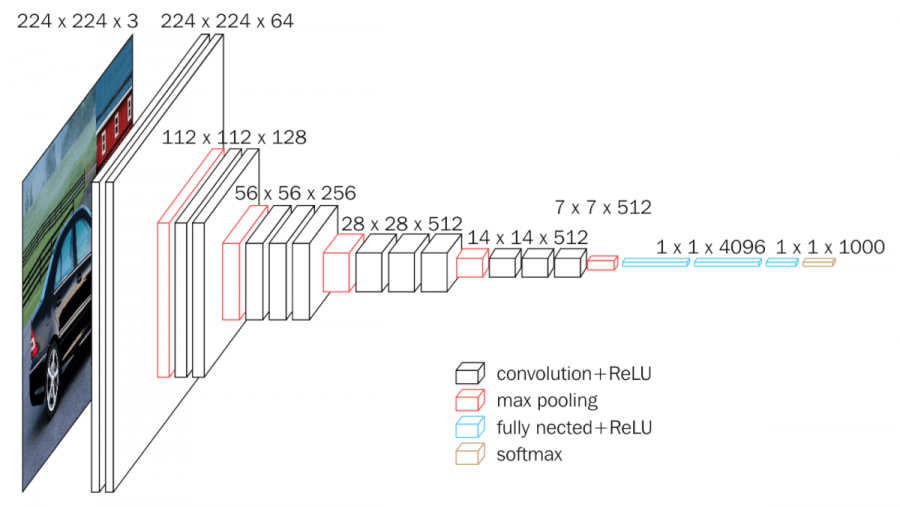
\includegraphics[width=0.8\textwidth]{Figures/vgg16}
  \caption{Structure of the VGG16 network.}%
  \label{fig:vgg16}
\end{figure}
This network was used to classify images with 1000 classes; this is why the
output is $1 \times 1 \times 1000$\footnote{The training data is labelled using
  one-hot encoding. This means the to each image a $1000$ dimensional vector is
  associated where each component corresponds to one class that we want to
  predict and that contains a $1$ in the corresponding entry and is zero
  everywhere else. The network will usually not be 100\% certain about its
  decision and thus the final output of the layer will be a $1000$ dimensional
  vector of which the entries sum to one and which has large values in the
  components that correspond to the predicted classes.}. To gradually reduce the
spatial dimension from $224 \times 224$ to $1 \times 1$, so called max pooling
layers are used.  In this particular case $2 \times 2$ max pooling with a stride
of $2$ was used, which means that the image is partitioned into $2 \times 2$
blocks of which the maximum of the respective four values is taken to replace
this block. The result is a smaller image, more precisely the spatial dimension
is reduced by two in each direction. The effect is visualised in the Figure
below.
\begin{figure}[H]
  \centering 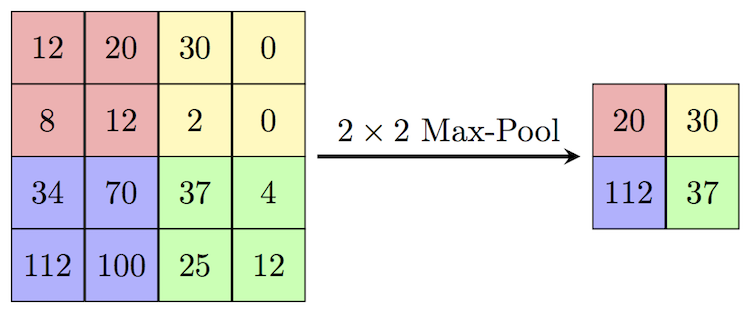
\includegraphics[width=0.6\textwidth]{Figures/maxpool}
  \caption{Effect of a $2 \times 2$ max pool.}%
  \label{fig:maxpool}
\end{figure}
Most layers of the network are convolutional layers with a small receptive field
of $3 \times 3$. For instance, the first two layers after the input layer
consist of 64 distinct convolution filters (typically, in these early layers,
these are edge detectors and the like).

After the stack of convolutional layers, three fully connected layers are
trained. The first two have 4096 channels each, which results in
$4096 \times 4096$ parameters that need to be trained (which is much more than
the number of parameters in the convolutional layers). At the end of
Section~\ref{sec:unet} we compute the total number of a CNN in more detail.

The non-linearity used in all of the hidden layers was a rectified linear unit
(ReLU). The last layer consists of a so called softmax function. The goal of
this function is as follows. Prior to applying softmax, some vector components
could be negative, or greater than one; and might not sum to 1; but after
applying softmax, each component will be in the interval $(0,1)$ and the
components will add up to 1, so that they can be interpreted as
probabilities. Furthermore, the larger input components will correspond to
larger probabilities.

\section{Training of a Neural Network: Optimisation}%
\label{sec:train_cnn}
When we have decided on which architecture we want to use (cf.~the last
chapter), we can start to train the network. We begin by initialising the
weights randomly which will obviously not generate any meaningful results.  The
goal is now to (iteratively) find a set of weights that correspond to a
better-performing network, or in other words weights that correspond to a lower
loss. Most modern network use the (stochastic) gradient descent algorithm to
minimise the loss function. To find a minimum of a function starting from a
random point on the graph, we can go in the direction of a negative gradient.
This is the basic idea of gradient descent. At each step in learning we go one
step in the direction of a negative gradient; of course theoretically the
derivative only guarantees that the function will decrease if we take an
infinitely small step which is obviously not possible in practice. The ``size''
of the step is a hyper-parameter called the learning rate which has to be
adjusted beforehand.

In classic gradient descent, we would do this for every image in the training
set which is usually very inefficient. Especially in the beginning, where the
weights have random values, it is not necessary to incorporate every training
image in computing the next (small) step towards a minimum. Therefore we only
optimise over so called mini-batches of the dataset which are usually chosen
randomly from the set of training images. The size of the mini-batch is another
hyper-parameter that has to be chosen before training; usually batches are not
larger than 100 (in some contexts only the extreme case of mini-batches
consisting o a single image is called stochastic gradient descent; sometimes
also mini-batch gradient descent is referred to as stochastic gradient descent).

\section{Convolutional Neural Networks for Semantic Segmentation}%
\label{sec:unet}%
The goal of semantic segmentation is to understand what is in an image on a
pixel level, \ie to assign a class to each pixel in an image. This is visualised
in the following image which is taken from the CityScapes dataset.
\begin{figure}[H]
  \centering 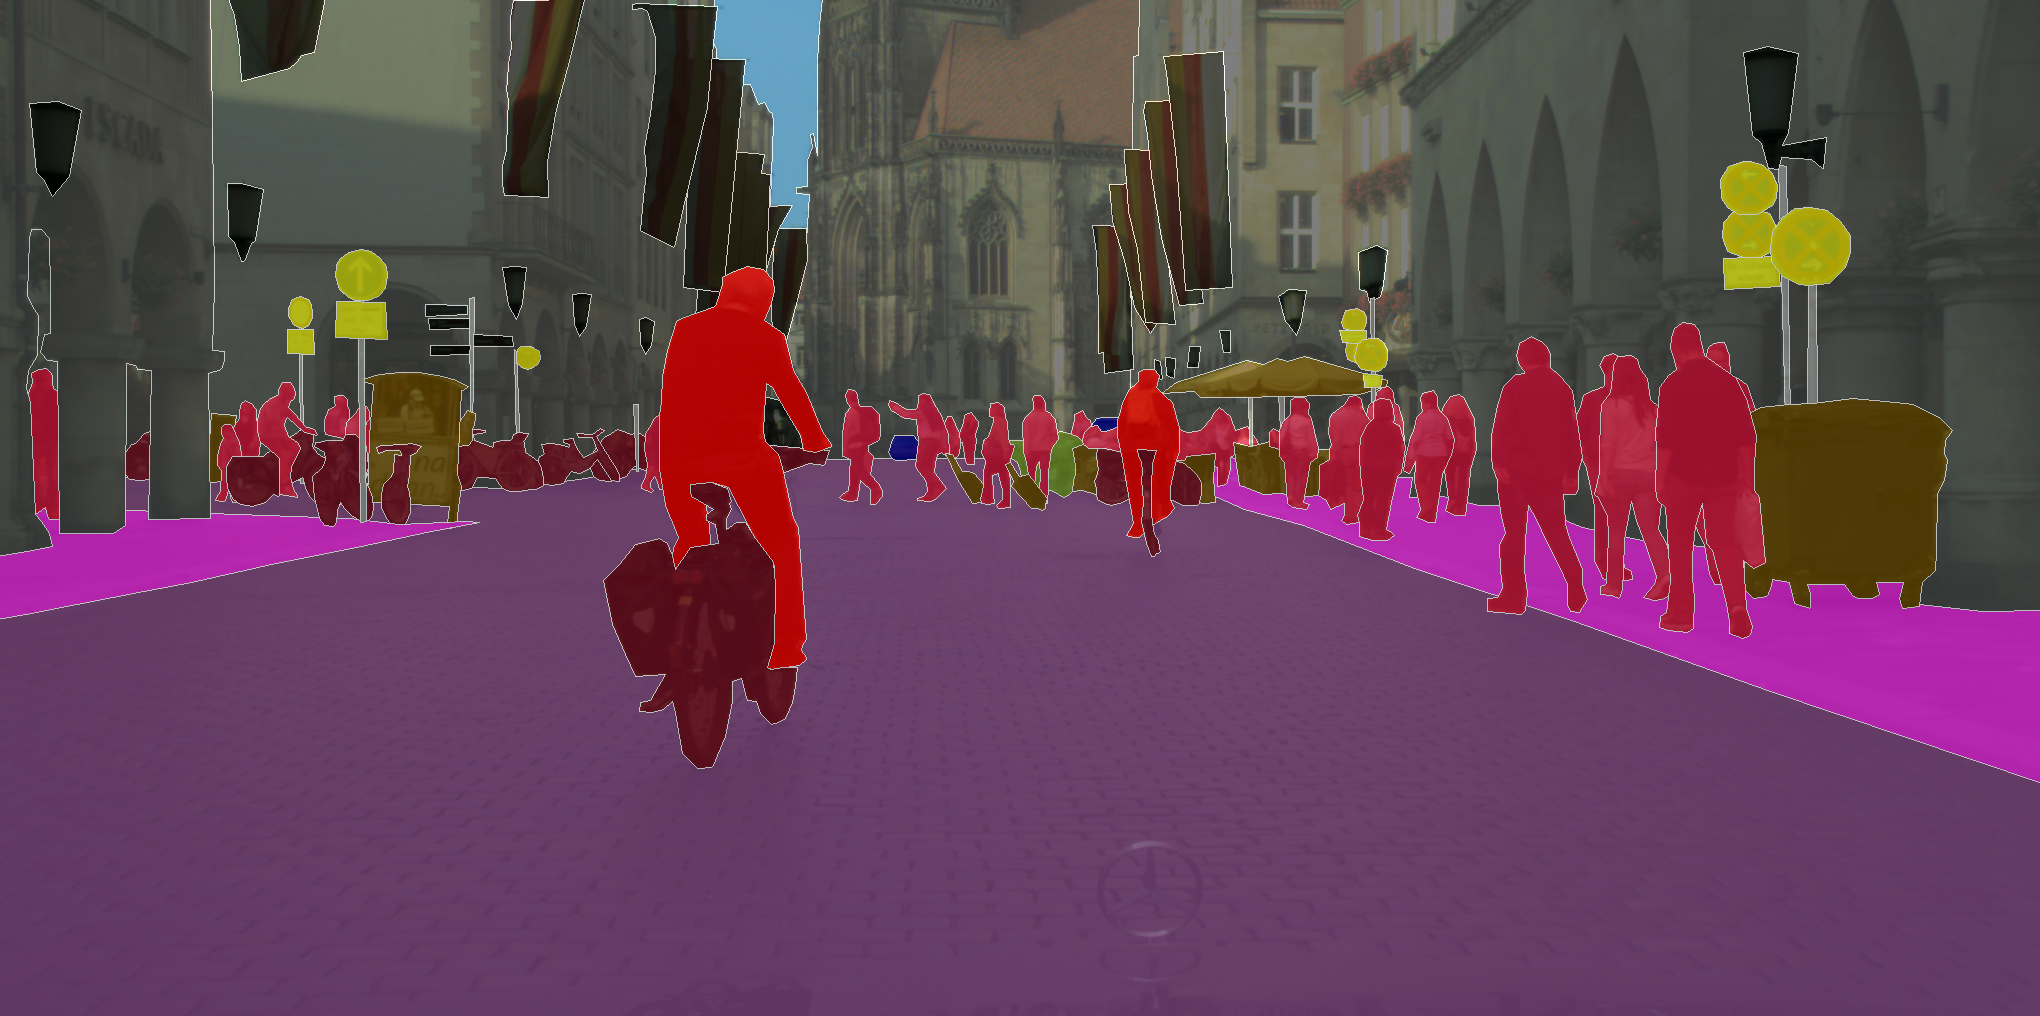
\includegraphics[width=0.7\textwidth]{Figures/cityscapes}
\end{figure}
Another application of semantic segmentation is pose estimation. Here, the
network is asked to find, for instance, all left hands in an image, or all right
feet etc.

One very famous and very successful architecture of a CNN for semantic
segmentation is the UNet given in Figure~\ref{fig:unet}.
\begin{figure}[htpb]
  \centering 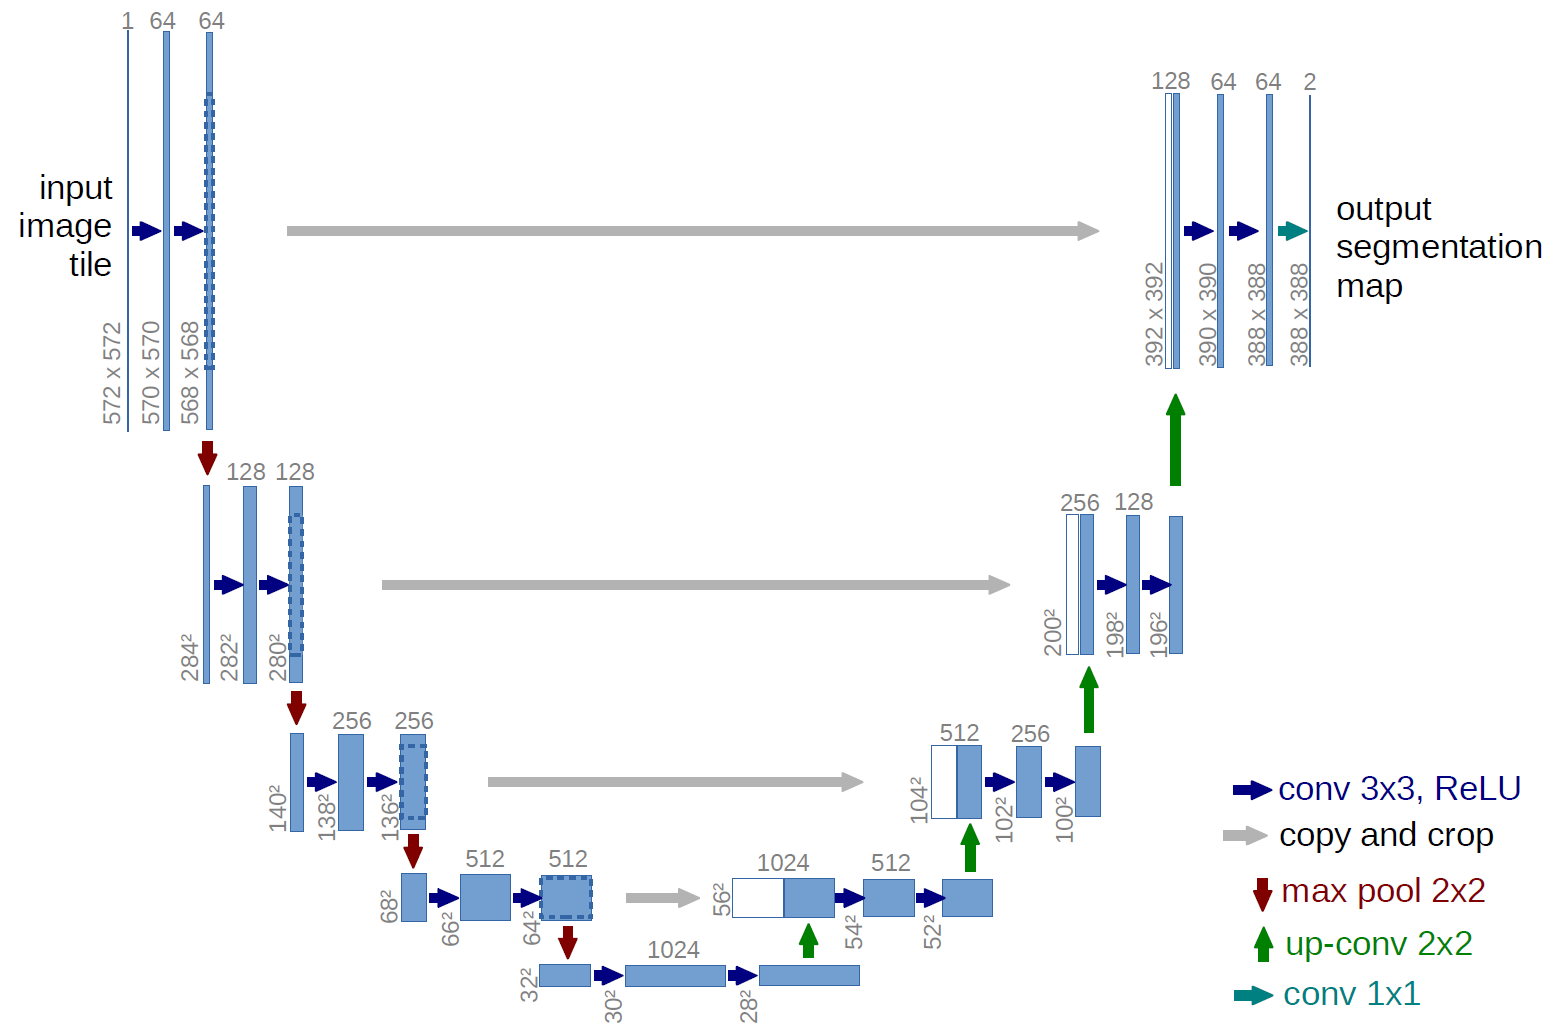
\includegraphics[width=0.7\textwidth]{Figures/unet}%
  \caption{Architecture of the UNet}%
  \label{fig:unet}
\end{figure}
One main difference when compared to the networks we previously discussed is
that some layers or not only connected to the previous layer but also to other
layers. More precisely, the output of some of the early layers is fed into the
corresponding late layer of the same resolution. Further, instead of using max
pool to reduce the dimensions of the image, smoothing and downsampling
convolutional filters are used. They are not prespecified to a certain filter
but are also learned. Similarly, upsampling convolution filters are used to
increase the dimension again. The approach of the UNet can be interpreted as
follows. The layers on the bottom in the Figure are very low-resolution but have
many channels (up to 2014). The path through these layers is therefore referred
to as the semantic pathway. Due to the high number of channels, its aim is to
learn \emph{what} is in each part of the image. However, the low resolution of
$\sim 30 \times 30$ prohibits the network form learning exactly \emph{where}
these things are (for example in the CityScapes dataset, the network might be
very certain that somewhere in the left side of the image there is a tram but it
is unable to exactly pin down its location). This is where the skip connections
(grey, from left to right) come into play. Although they obviously have not yet
understood the difference between, \eg, a tram and a pedestrian, they have
learned where the boundaries of each of these objects are, as they typically act
as edge detectors. This information from this so called geometric pathway is
then combined with the information from the semantic pathway.

In practice, there are several techniques that should be used to improve the
performance of the UNet. First, one should definitely use some form of
normalisation, either group or batch norm (described below). Also, residual
connections should be used in each of the individual blocks of the UNet. A
simple schematic is given in Figure~\ref{fig:resblock}. In addition to the
output from the previous layer, also the output of the layer before that is fed
into Layer I. While one could use certain linear transformations to transform
the skip connection, often the two outputs are simply added to form the new
input. This is sometimes referred to as a highway network. For more layers
inside a block, additional connections are added. For instance, in a block of
four layers, also the output of the second layer would be fed into the fourth.
Furthermore, one could also add second-order connections, \ie in the example of
four layers, one could connect the first and fourth layer, skipping two layers
instead of just one. In practice, these residual connection made it possible to
train very deep network with 50--100 layers.

\begin{figure}[htpb]
  \centering
  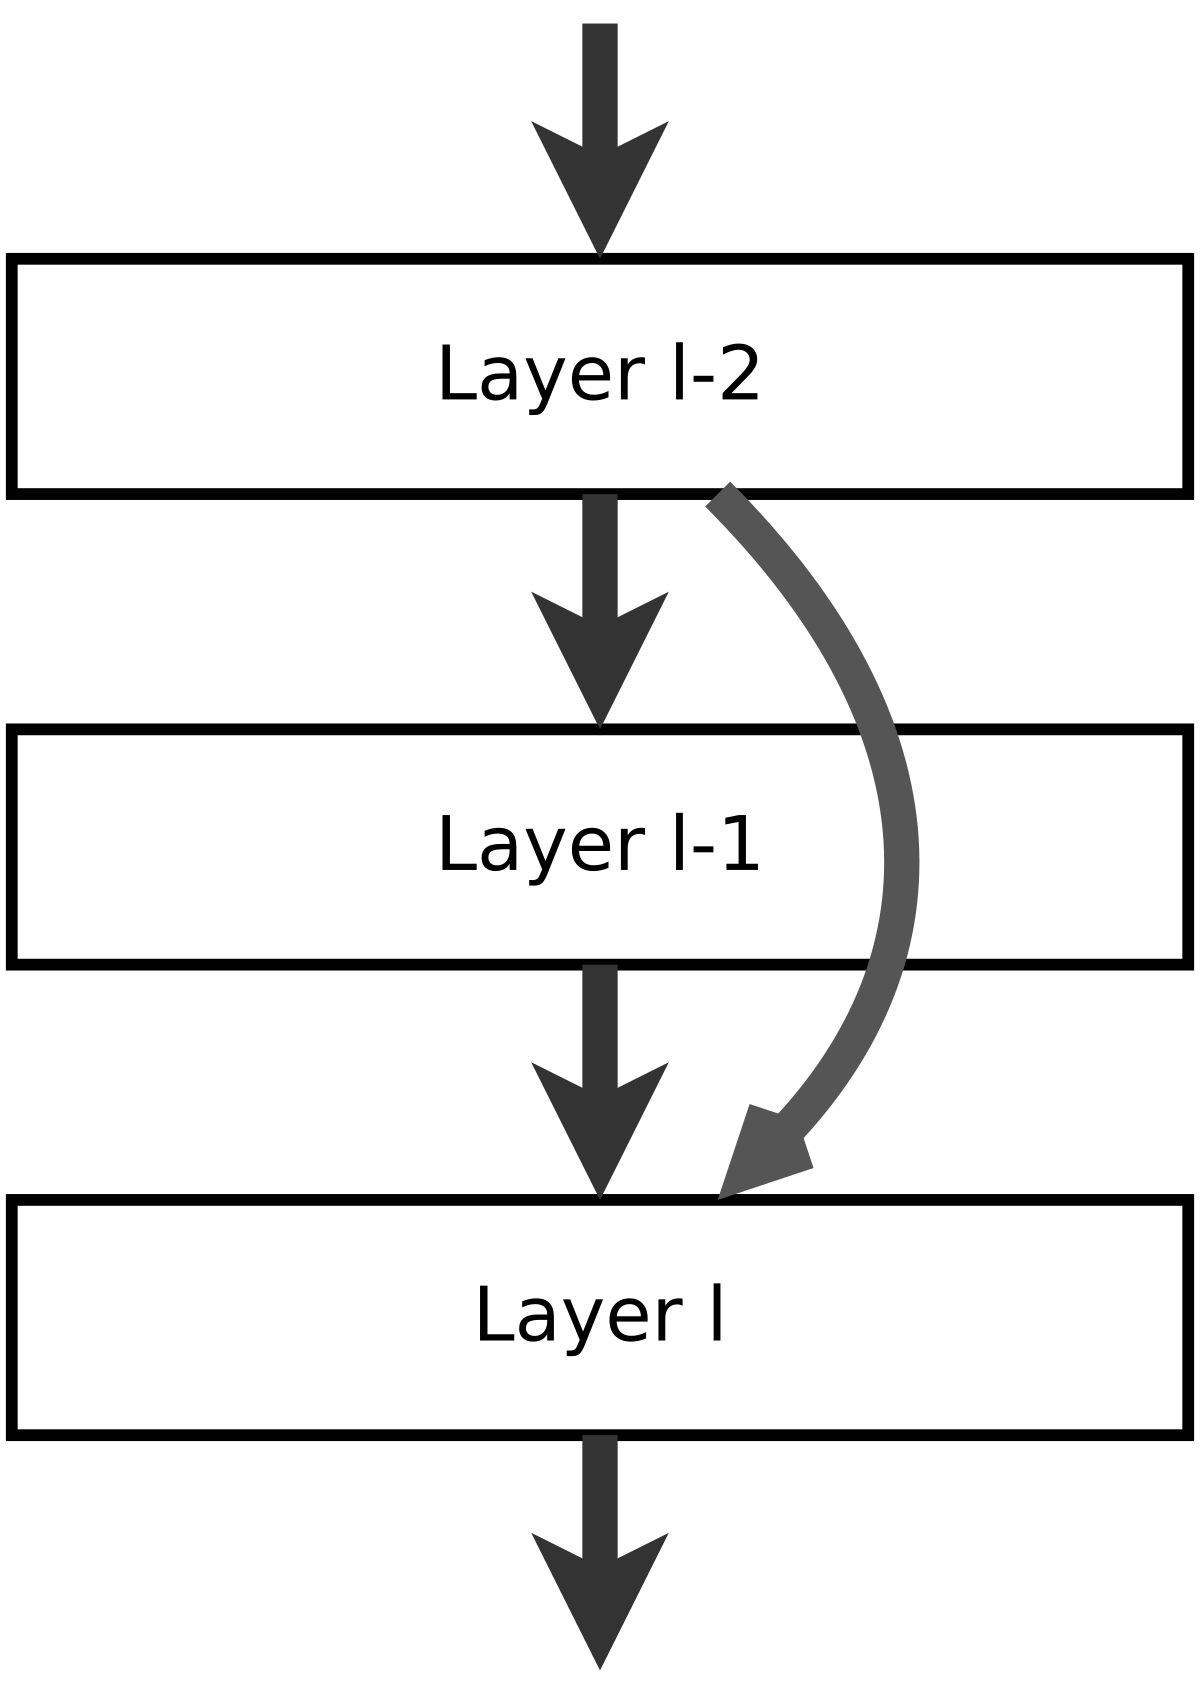
\includegraphics[width=0.3\textwidth,angle=90,origin=c]{Figures/resblock}
  \caption{Residual block with an additional connection from the layer before
    the previous layer.}%
  \label{fig:resblock}
\end{figure}

\subsection*{Batch and Group Normalisation}
Batch normalisation is a method that normalises activations in a network across
the current mini-batch. For each feature, batch normalisation computes the mean
and variance of that feature in the mini-batch. It then subtracts the mean and
divides the feature by its mini-batch standard deviation. After the
normalisation, the activations have zero mean and unit standard deviation. In
practice it was observed that batch normalisation has a huge impact on the
effectiveness of the training of the network. Although there are many
contributions discussing the actual effect of batch normalisation and explaining
why it works so well, it is not fully understood.

With very large networks, the size of the mini-batches is often restricted by
the available GPU memory and in the extreme case of a batch size of one, batch
normalisation is obviously useless (also, for very small batch sizes batch
normalisation does not work very well either). There is a variety of other
normalisation techniques, on more recent one being group normalisation. Here,
the mean and standard deviation are computed over groups of channels for each
training example. In particular for cases where batch norm was not applicable,
group norm has shown to produce very good results.

\subsection*{Performance measures}
We will now briefly discuss the importance of choosing a meaningful performance
measure to evaluate the performance of a neural network that is used for
semantic segmentation. A simply straightforward measure is the \emph{accuracy}
of the predictions. We simply compare the prediction and the corresponding
ground truth on a pixel wise basis.  The ratio of correctly classified pixels
divided by the number of total pixels then gives the accuracy. This, however,
has one big flaw. Typically, the majority of an image consists of background,
say 90\% percent, and the remaining 10\% consist of the pixels that we want to
classify into different classes. If we now simply classify each pixel in our
prediction as background, we have an accuracy of 90\% although our prediction is
completely meaningless. Thus, we require a performance measure that incorporates
the fact that much of the image is background, \ie that specifically ``targets''
pixels in the foreground class. One that is widely used is the
\emph{intersection over union} or IoU, for short.

It is based on the following idea. Suppose we have some object that we want to
recognise in the image, say a cat. Now we use the network to predict the
location of the cat, \ie we have a certain region of pixels classified as cat.
If the prediction was perfect, the classified pixels and the corresponding
ground truth would completely overlap. This is unlikely in practice, but this
intersection should be maximised. At the same time we want to reduce the false
positive errors, \ie the pixels classified as cat that do not belong to the cat.
We of course also want to reduce the false negative errors, \ie the pixels that
belong to the cat but are not classified as such. Thus, to evaluate how good of
a prediction that network has made, we divide this intersection by the area of
cat in the ground truth and in our prediction, \ie the union between both. In
summary, we compute the ratio between the intersection and the union, or the
intersection over union. If we know simply classify everything as background,
the intersection between classified pixels and ground truth is empty and thus
the IoU score of this prediction would be zero, which much better represents the
quality of the prediction.

\subsection*{Number of Parameters and the Receptive Field of a CNN}
To finish this chapter we will discuss how the total number of parameters of a
particular network can be computed and we will also introduce and compute the
notion of the receptive field. We consider the network given in
Figure~\ref{fig:cnn_arch}.

\begin{figure}[htpb]
  \centering 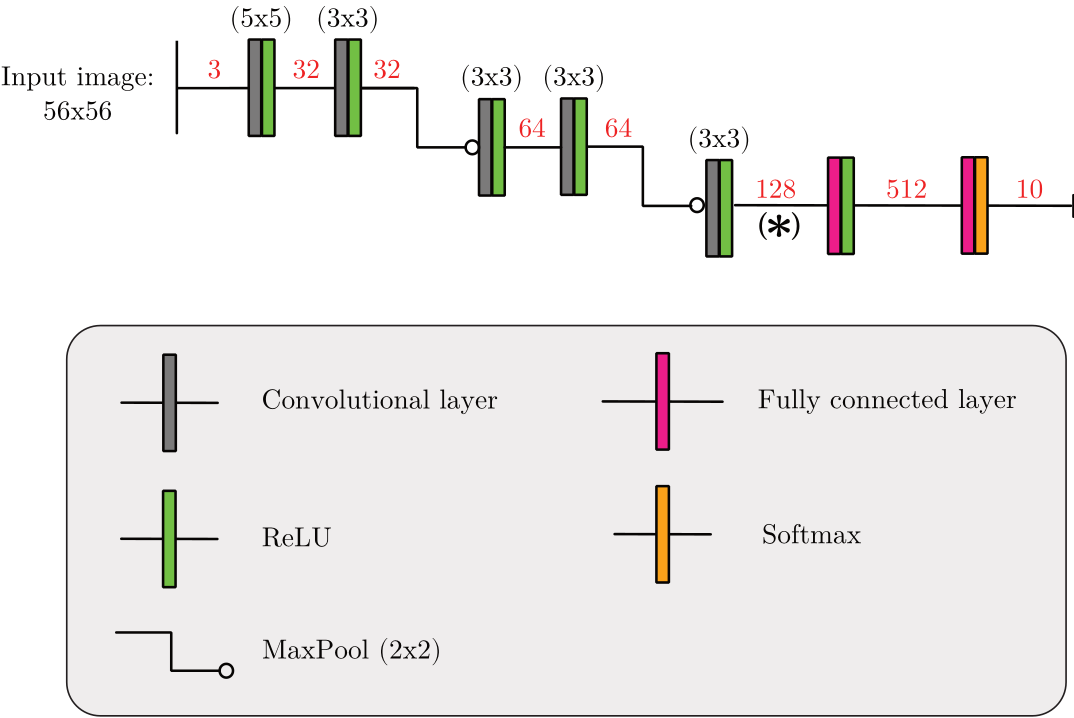
\includegraphics[width=0.8\textwidth]{Figures/cnn_arch}
  \caption{Example of very simple architecture for image classification. The
    input is an RGB image (three channels) with size $56\times 56$. The numbers
    of channels are written in red: the number of output classes is 10. For each
    convolution layer, the dimension of the 2D filter is specified. In the
    architecture we always use ``same'' convolutions, so that the input is
    padded with zeros and the convolution output has the same spatial
    dimension.}%
  \label{fig:cnn_arch}
\end{figure}

The only layers that contain learnable parameters are the convolutional layers
and the fully connected layers. If the filter inside a convolutional layer has
size $k \times k$ and the filter has $in$ input and $out$ output channels, we
have a total of $in \cdot k \cdot k \cdot out$ parameters. In a fully connected
layer, the number of parameters is simply $in \cdot out$. Note, however that in
this case, the number $in$ depends on how the network has previously altered the
input size, \eg by max-pool layers. We begin by computing the number of
parameters for each of the convolutional layers and add them up:
\begin{equation*}
  3 \cdot 5 \cdot 5 \cdot 32 + 32 \cdot 3 \cdot 3 \cdot 32 + 32 \cdot 3 \cdot 3 \cdot 64 + 64 \cdot 3 \cdot 3 \cdot 64 + 64 \cdot 3 \cdot 3 \cdot 128\,,
\end{equation*}
which yields a total of $140.640$ parameters in the convolutional layers. To
compute the number of parameters in the fully connected layers, we first have to
calculate the size of the input at the output of the convolutional part of the
model, which is indicated with $(\ast)$ in the Figure. Since we are using same
convolutions, the only layers that alter the size of the input are the
$2 \times 2$ max-pool layers. Each of these layers reduces the size of the input
by $2$ along each axis. Since we have two of these layers in the network, the
input size at $(\ast)$ is $14 \times 14$ since $56 / 2 / 2 = 14$. Since we have
$128$ input channels, the total number of inputs of the first fully connected
layer is $14 \cdot 14 \cdot 128 = 25088$ and consequently the number of
parameters in the first fully connected layer is $25088 \cdot 512$. The number
of parameters in the second fully connected layer is simply given by
$512 \cdot 10$, which results in a total of $12.850.176$ parameters. All
together, the network has $140.640 + 12.850.176 = 12.990.816$ learnable
parameters.\footnote{Actually, the number is even slightly higher since we
  neglected the so called bias terms.} We see that in general, fully connected
layers involve many more parameters as compared to convolutional ones.

We will now discuss the notion of the receptive field and compute the receptive
field of the CNN from Figure~\ref{fig:cnn_arch} at the output of the
convolutional layer, marked with $(\ast)$. The receptive field is defined as
that part of the input image that a particular feature of the CNN is affected
by. In a fully connected layer, each neuron is connected to each neuron of the
previous layer. Consequently, each feature in the input has some influence on
every feature of the output. With a convolutional layer this is obviously not
the case. If the convolution filter is of size $3 \times 3$, the output features
are affected by $9$ of the input features. Now, if we feed this output again
into another convolutional layer, the convolution operation there will combine
features that have themselves been computed by different parts of the input
image. Thus, the receptive field was increased since each output of this layer
is affected by a larger number of input features than the previous layer.

To compute the receptive field we go backwards through the network starting from
the location at which we want to compute the receptive field. Each convolutional
layer with a kernel of size $2h+1 \times 2h+1$ will increase the receptive field
by $2h$ in each direction.  Similarly, each max pool layer with size
$2 \times 2$ will double the receptive field. We want to know by how many pixels
of the input one pixel (or a patch of size $1 \times 1$) of the output of layer
five is affected. Thus we begin with this pixel, adding two for the
convolutional layer (layer V), multiplying this value by two to account for the
max pool, then again adding two for layer IV etc. This yields
\begin{equation*}
  (((1 + 2) * 2) + 2 + 2)*2 + 2 + 4 = 26\,,
\end{equation*}
thus the receptive field is $26 \times 26$ (since all convolutional layers are
symmetrical).

%%% Local Variables:
%%% mode: latex
%%% TeX-master: "../main"
%%% End:
